\chapter{The Question of Transformation}

This chapter begins before the dialogues themselves begin. The source is the Krishnamurti Foundation Trust material, curated by LazyingArt LLC through Video2Book, and the setting is Brockwood Park. What we have here is not a blackboard lecture and not a formal derivation. It is the opening alignment of three lines of inquiry: David Bohm's physics, David Shainberg's psychiatry, and Krishnamurti's demand that the inquiry come down to actual daily life. The displayed formulas in this chapter are therefore not recovered board equations. They are deliberately modest structural notation, used to keep the movement of the conversation clear without inventing mathematics that the source does not contain.

\section{Before The Dialogues Begin}

The first question asks for background before the dialogues begin. Where are we? Who is speaking? How did these participants come to take part with Krishnamurti? That opening may look merely introductory, but it sets the method of the whole inquiry. We do not begin with a doctrine. We begin with a place, a group of people, and the histories that brought them into contact.

Bohm first locates the discussion at Brockwood Park in Hampshire, England. He then identifies himself as a professor of theoretical physics at the University of London. That professional identity matters because it gives his entry into Krishnamurti's work a particular weight. But the lecture immediately turns from title and position to motive. Bohm wants to explain not only who he is, but why this inquiry touched something already alive in his work.

A compact way to mark the opening arrangement is
\begin{equation}
\text{Brockwood Park}
\quad\longrightarrow\quad
\{\text{physics},\ \text{psychiatry},\ \text{Krishnamurti's inquiry}\}.
\end{equation}
This is not a formula in the physical sense. It is a map of the room: several disciplined approaches to life are about to meet, and the chapter must let that meeting unfold in order.

\section{Bohm's Deeper Questions}

Bohm says that in theoretical physics he had always been interested in what he calls the deeper questions: the nature of time and space, space and matter, causality, what is behind it all, and what is universal. We should hear this carefully. He is not presenting a technical physics result. He is describing a pressure inside physics itself, a dissatisfaction with merely calculational success when the deeper order of things remains obscure.

We can gather this field of concern as
\begin{equation}
\mathcal{Q}_{\mathrm{Bohm}}
=
\{\text{time},\ \text{space},\ \text{matter},\ \text{causality},\ \text{universality}\}.
\end{equation}
The notation \(\mathcal{Q}_{\mathrm{Bohm}}\) is editorial. It names the cluster of questions that prepared Bohm to recognize something in Krishnamurti's work. The point is not that Krishnamurti gave Bohm a physics equation. The point is that Bohm's own discipline had already led him toward questions that were not merely technical.

The next movement is biographical, but it is still part of the argument. In Bristol, in 1957, Bohm and his wife went to the public library and became interested in books on philosophy and religion. They picked up Krishnamurti's \emph{The First and Last Freedom}. Bohm found it especially interesting because it discussed the observer and the observed.

\section{The Observer And The Observed}

The observer and the observed form the first conceptual hinge of the lecture. Bohm says this issue is significant in theoretical physics and quantum theory, and he refers to Heisenberg's bringing out the effect of the observer on the particle observed. The source gives no uncertainty relation, no wavefunction, and no operator formalism. We should not supply one. But we should preserve the exact importance of the remark: Bohm recognizes a structural problem that physics had already forced into view.

For Bohm's physics-facing reference, we may write the cautious schematic
\begin{equation}
\text{observer}
\quad\longrightarrow\quad
\text{observed particle}.
\end{equation}
The arrow means involvement, effect, or disturbance. It is not a measurement operator and not a hidden derivation. It simply marks the fact that observation is not always external to what is observed.

The phrase that becomes decisive for the larger Krishnamurti inquiry is stronger:
\begin{equation}
\text{observer} = \text{observed}.
\end{equation}
This, too, is not a mathematical identity. It is a compact notation for a psychological and existential claim: the observer who looks at fear, desire, hurt, or fragmentation is not standing outside the field he observes. The observer is part of that field.

\subsection{Question \& Answer}

\paragraph{Question.}
Is Bohm only making an analogy between quantum theory and Krishnamurti's inquiry?

\paragraph{Answer.}
No technical analogy is established in the transcript. Bohm mentions quantum theory because the observer/observed question matters there, especially in relation to Heisenberg. But the lecture does not move from quantum mechanics into a theory of consciousness. It moves from a physicist's sensitivity to foundational questions into a broader human inquiry. The resemblance should be preserved, but not inflated.

The distinction is best kept in two lines:
\begin{align}
\text{physics reference:}\qquad
&\text{observer affects observed},\\
\text{Krishnamurti inquiry:}\qquad
&\text{observer is observed}.
\end{align}
The first line still allows a distance between observer and observed, even if the act of observing has an effect. The second line questions that distance itself. This is why the phrase can pass from Bohm's physics into Shainberg's psychiatry without becoming a piece of physics.

\section{From Reading To Relationship}

After this recognition, Bohm's account becomes a history of contact. The transcript is severely garbled for a short stretch after his remark that he read as many books as he could find, so we should not build detailed claims from that passage. The recoverable movement is clear: Bohm arranged to speak personally with Krishnamurti; they met and talked; Bohm told him about his ideas in physics; Krishnamurti appreciated the spirit of those ideas.

Then the rhythm becomes repeated contact. When Krishnamurti came to London, they arranged to meet. Later Bohm went to Saanen, where they met more often. Around 1966 or 1967, Krishnamurti asked him to take part in the plan for a school, and that school gradually became organized at Brockwood Park. Bohm became involved with the foundation responsible for the school and came regularly to discuss and take part.

The movement is worth displaying because it prevents us from treating the observer/observed question as a one-time intellectual coincidence:
\begin{equation}
\text{reading}
\longrightarrow
\text{conversation}
\longrightarrow
\text{repeated meetings}
\longrightarrow
\text{shared work at Brockwood}.
\end{equation}
The point of this sequence is continuity. A conceptual recognition became a relationship of inquiry.

\section{Shainberg And The Psychiatric Problem}

The interviewer then turns to David Shainberg. The structure repeats, but the discipline changes. Shainberg is a practicing psychiatrist in New York City. He came to read and think about Krishnamurti early, through the influence of his father and through his interest in psychoanalytic work associated with Karen Horney and Harold Kelman. Even then, he says, there seemed to be something important in the question that the observer is the observed.

The parallel with Bohm is useful, provided we do not flatten it. Bohm approaches through foundational physics. Shainberg approaches through psychiatry, neurology, psychoanalysis, and the practical problem of human suffering. We can set the entrances side by side:
\begin{equation}
\begin{array}{ccl}
\text{Bohm} &:& \text{physics} \longrightarrow \text{observer/observed},\\
\text{Shainberg} &:& \text{psychiatry} \longrightarrow \text{observer/observed}.
\end{array}
\end{equation}
The notation is schematic. It is meant only to preserve the lecture's structure: two very different disciplines converge on the same pressure point.

Shainberg's own path then widens. He goes through college, medical school, psychiatry, neurology, and psychoanalysis. All along he reads Krishnamurti and tries to understand the difference between what Krishnamurti is saying and what Western psychiatry or psychology communicates. Only in the more recent years, he says, had he begun to feel how it might enter his work, and much of that stimulus came from meeting Bohm.

\section{Fragmentation Treating Fragmentation}

Shainberg's central word is fragmentation. He says that psychological theories deal with fragmentation and with relationships between fragments, but that most of them do not understand the holistic action, or holism, that gives birth to this fragmentation. He then makes the sharper clinical point: theories that analyze and break things into pieces may collaborate with the very problems patients present.

Here the chapter can use a small worked schema. Suppose we start with a divided observer, someone who approaches suffering as though he were outside it. That observer produces a divided theory. The theory then treats fragmentation as an object over there. But if the observer is part of the observed field, the theory may reproduce the division it claims to treat:
\begin{align}
\text{fragmented observer}
&\longrightarrow
\text{fragmented theory},\\
\text{fragmented theory}
&\longrightarrow
\text{fragmentation treated as an object},\\
\text{fragmentation treated as an object}
&\longrightarrow
\text{possible continuation of fragmentation}.
\end{align}
This is not a formal psychological model. It is a faithful reconstruction of Shainberg's worry in logical order. The observer/observed problem has now left the realm of physics reference and entered the doctor-patient situation.

\subsection{Question \& Answer}

\paragraph{Question.}
Can a fragmented theory adequately understand fragmentation?

\paragraph{Answer.}
Shainberg's answer is not a simple no, but it is deeply cautious. His point is not that analysis is useless or that psychiatry should be discarded. His point is that when the theorist is fragmented, and when the theory is itself a product of that fragmentation, the theory may represent fragmentation and then call that representation the thing to be treated. The danger is circular.

We can write the danger compactly:
\begin{equation}
\text{fragmented observer}
+
\text{fragmented theory}
\not\Rightarrow
\text{freedom from fragmentation}.
\end{equation}
The symbol \(\not\Rightarrow\) carries only its ordinary logical force: the conclusion does not follow. The lecture does not prove a theorem. It opens a problem that the later dialogues are meant to examine.

\begin{figure}
\centering
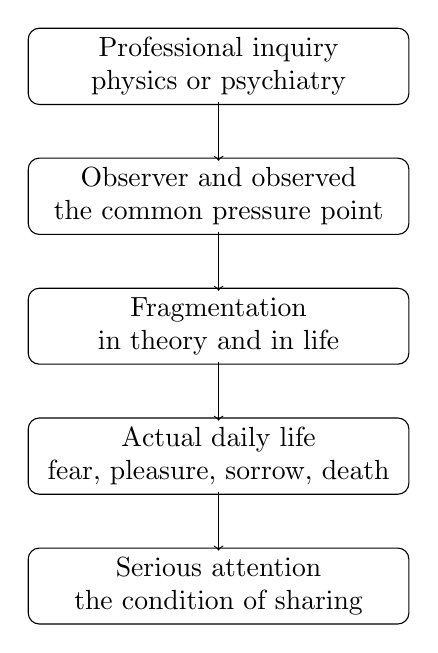
\begin{tikzpicture}[x=1cm,y=1cm]
\node[draw, rounded corners, align=center, text width=4.6cm] at (0,0) {Professional inquiry\\physics or psychiatry};
\node[draw, rounded corners, align=center, text width=4.6cm] at (0,-1.65) {Observer and observed\\the common pressure point};
\node[draw, rounded corners, align=center, text width=4.6cm] at (0,-3.30) {Fragmentation\\in theory and in life};
\node[draw, rounded corners, align=center, text width=4.6cm] at (0,-4.95) {Actual daily life\\fear, pleasure, sorrow, death};
\node[draw, rounded corners, align=center, text width=4.6cm] at (0,-6.60) {Serious attention\\the condition of sharing};
\draw[->] (0,-0.45) -- (0,-1.20);
\draw[->] (0,-2.10) -- (0,-2.85);
\draw[->] (0,-3.75) -- (0,-4.50);
\draw[->] (0,-5.40) -- (0,-6.15);
\end{tikzpicture}
\caption{A transcript-based map of the introductory movement. No validated blackboard diagram exists for this lecture; the figure is an editorial aid.}
\end{figure}

\section{Krishnamurti's Demand For Seriousness}

The interviewer finally turns to Krishnamurti and asks how the viewer can best share in these dialogues. Krishnamurti's answer changes the level of the discussion. He does not ask whether the viewer has mastered physics, psychiatry, or the history of Brockwood Park. He says it depends on how serious one is: how deeply one wants to go into these questions, which are, after all, one's life.

This is the decisive pivot. The dialogue is not about theoretical abstraction. Krishnamurti says they are dealing with actual daily life, wherever one lives. He names the facts of fear, pleasure, sorrow, death, and the question of whether there is anything sacred in life. We can collect that field as
\begin{equation}
\mathcal{A}
=
\{\text{fear},\ \text{pleasure},\ \text{sorrow},\ \text{death},\ \text{the sacred}\}.
\end{equation}
Again, \(\mathcal{A}\) is not a technical classification. It is a way of keeping before us the concrete field Krishnamurti names. The inquiry has not become less exact by leaving professional theory. It has become more exact, because it now has to touch the facts of life directly.

Krishnamurti's position can be stated as a proposition.

\begin{proposition}
To share in the dialogue is not primarily to agree with it, believe it, or interpret it from a distance. It is to bring seriousness, care, and attention to the actual facts of one's own life.
\end{proposition}

\begin{proof}
The viewer asks how to gain the most from the dialogues. Krishnamurti answers by making seriousness the condition. He then distinguishes the inquiry from abstract hypothesis and names actual daily life as its field. Therefore the relevant participation is not passive reception or theoretical commentary. It is attention to the facts under discussion.
\end{proof}

The word attention should remain precise. It is not a method being sold, and it is not a mood of inspiration. In this opening, attention belongs with care and seriousness. Without something real, something true, Krishnamurti says, life has very little meaning. That is why the chapter cannot end in biography. It has to end where the lecture ends: with the demand that the listener enter the inquiry directly.

\section{Summary}

The lecture's movement is simple, but it should not be compressed too aggressively. Bohm enters through theoretical physics and the deeper questions of time, space, matter, causality, universality, and the observer/observed relation. Shainberg enters through psychiatry and the problem that fragmented theories may collaborate with fragmentation. Krishnamurti then redirects both lines of approach toward actual daily life.

The chapter therefore preserves three movements:
\begin{enumerate}
\item From physics to the question of the observer and the observed.
\item From psychiatry to the problem of fragmentation treating fragmentation.
\item From professional theory to serious attention to fear, pleasure, sorrow, death, and the sacred.
\end{enumerate}
There are no validated screenshots or blackboard equations for this lecture, so the displayed formulas and the diagram remain subordinate to the spoken source. Their purpose is to make the structure legible. The real spine of the chapter is the turn from explanation to seriousness: if we are to enter these dialogues, we must do so because the subject is our own life.